\documentclass[11pt,letterpaper]{article}
\usepackage[hmargin=1in,top=.94in,bottom=.95in]{geometry}
\usepackage{amsmath,amssymb,amsthm,mathtools}
\usepackage{graphicx,booktabs}
\usepackage[hidelinks]{hyperref}
\setcounter{tocdepth}{1}
\setlength{\emergencystretch}{1.6em}
\newtheorem{theorem}{Theorem}[section]
\newtheorem{lemma}[theorem]{Lemma}
\newtheorem{proposition}[theorem]{Proposition}
\newtheorem{corollary}[theorem]{Corollary}
\theoremstyle{definition}
\newtheorem{definition}[theorem]{Definition}
\numberwithin{equation}{section}
\DeclareMathOperator{\Tr}{Tr}
\DeclareMathOperator{\rank}{rank}
\DeclareMathOperator{\ran}{ran}
\newcommand{\R}{\mathbb R}
\newcommand{\C}{\mathbb C}
\newcommand{\F}{\mathbb F}
\newcommand{\N}{\mathbb N}
\newcommand{\Q}{\mathbb Q}
\raggedbottom
\setlength{\intextsep}{10pt plus 2pt minus 2pt}
\setlength{\textfloatsep}{13pt plus 2pt minus 2pt}
\makeatletter
\renewcommand{\maketitle}{\begin{center}{\LARGE\@title\par}\end{center}\vspace{.25em}}
\makeatother
\title{Exact Stabilizer Membership for Low-Rank Density Matrices}
\author{}
\date{}
\begin{document}
\maketitle
\begin{abstract}
Let \(\rho\) be an explicitly given \(D\times D\) qubit density matrix over \(\Q(i)\), of ordinary rank \(r\) and input bit length \(L\). We decide membership in the stabilizer polytope in \(2^{O(\log^2(r+1))}\operatorname{poly}(D,L)\) bit operations. A Pauli averaging argument yields a postselection that is injective on the support of \(\rho\) whenever \(D>r^2\). Iteration reduces the search for stabilizer rays to a space of dimension at most \(r^2\). The algorithm returns either a rational convex decomposition with at most \(r^2\) terms or a rational Hermitian witness valid on every stabilizer state. A family of coordinate subspaces attains the quadratic scale of the one-step obstruction. We also give an exact decision algorithm for odd prime local dimension.
\end{abstract}
\section{Introduction}
A mixed state is free in the stabilizer theory of magic precisely when it belongs to the convex hull of the pure stabilizer projectors. An \(n\)-qubit system has \(2^{\Theta(n^2)}\) stabilizer vertices. A density matrix of small rank lies on a face of the positive semidefinite cone, and every vertex appearing in a positive decomposition must lie on that same face. The computational question is how to find those vertices from a basis of the support.

\begin{theorem}\label{thm:qubit}
Let \(D=2^n\), and let \(\rho\in M_D(\Q(i))\) be an explicitly encoded density matrix of rank \(r\ge1\). With \(L\) the total binary encoding length, stabilizer membership is decidable deterministically in
\[
2^{O(\log^2(r+1))}\operatorname{poly}(D,L)
\]
bit operations. For a member the algorithm returns at most \(r^2\) stabilizer projectors and rational probabilities. For a nonmember it returns \(W=W^*\in M_D(\Q(i))\) with \(\Tr(W\rho)<0\) and \(\langle s,Ws\rangle\ge0\) for every stabilizer vector \(s\).
\end{theorem}
In particular, for every fixed \(c\), explicit inputs with \(r\le2^{c\sqrt n}\) admit a polynomial-time algorithm. The parameter \(r\) is the matrix rank of the input. A pure state has \(r=1\) regardless of how many stabilizer vectors are required to express it as a superposition.

\section{Related work}
Dehaene and De Moor described qubit stabilizer amplitudes by affine supports and quadratic phases~\cite{ddm}. This description permits exact enumeration and recognition of pure states. Bravyi et al.\ use decompositions into stabilizer vectors to simulate circuits~\cite{bravyi}. For mixed states, Leone and Bittel analyze convex-roof stabilizer entropies and their numerical evaluation at low rank~\cite{lb}. Leone, Eisert and Oliviero give a worst-case hardness result for weak membership in the full stabilizer polytope under the exponential time hypothesis~\cite{leo}. Our decision problem uses explicit exact matrix entries. Its dependence on the matrix rank comes from compressing the entire support before enumerating pure stabilizer states.

\section{An injective Pauli measurement}
Write \(\mathcal P_n=\{I,X,Y,Z\}^{\otimes n}\) for the \(D^2\) Hermitian Pauli representatives. Let \(S\subset\C^D\) have dimension \(r\), and let \(\Pi\) be its orthogonal projector. We use \(\|\cdot\|_F\) for the Hilbert--Schmidt norm.
\begin{lemma}\label{lem:average}
If \(D>r^2\), some nonidentity \(P\in\mathcal P_n\) has both outcome projections \((I\pm P)/2\) injective on \(S\).
\end{lemma}
\begin{proof}
In the Pauli expansion of a matrix \(A\), averaging \(PAP\) over \(P\) cancels every nonidentity coefficient. Hence
\[
\sum_{P}P\Pi P=Dr I,\qquad
\sum_{P}\|\Pi P\Pi\|_F^2
 =\sum_{P}\Tr(\Pi P\Pi P)=Dr^2 .
\]
Some summand is strictly less than one. The identity contributes \(r\), so the corresponding \(P\) is nonidentity. A unit \(P\)-eigenvector in \(S\), of either sign, would give \(\|\Pi P\Pi\|_{\rm op}\ge1\), whereas the operator norm is bounded by the Frobenius norm. The kernels in \(S\) of both outcome projections are therefore zero.
\end{proof}
A Clifford change of coordinates identifies either eigenspace with \(\C^{D/2}\). Compose this decoding with a chosen outcome projection. Stabilizer measurement takes each stabilizer ray either to a stabilizer ray or to zero~\cite{ddm,bravyi}. Injectivity rules out zero on \(S\).

Given a rational basis matrix for \(S\), scan the Pauli labels and outcomes, and retain the first decoded matrix of rank \(r\). The averaging lemma proves termination while \(D>r^2\). This procedure requires no numerical test on norms. A diagonal Pauli selects rows of one parity. For a Pauli with nonzero bit shift \(a\), a binary change of coordinates pairs indices \(x,x+a\). Decoding replaces each pair by a sum with relative phase in \(\{1,-1,i,-i\}\). This follows by writing \(P|x\rangle=\xi_x|x+a\rangle\), using \(\xi_{x+a}=\overline{\xi_x}\), and representing an eigenvector by its entries on one transversal of the pairs. The transversal is a binary hyperplane. The change of coordinates and the phase correction are Clifford operations, up to the common scalar of the selected branch.

Iteration gives a linear map
\begin{equation}\label{eq:compress}
 C:S\longrightarrow\C^{D'},\qquad
 \ker C=0,\qquad D'=2^m\le r^2 ,
\end{equation}
which preserves stabilizer rays on its domain. The rank remains \(r\) throughout. A common integer denominator clears a basis taken from independent columns of \(\rho\). In these unnormalized coordinates each measurement at most doubles the largest modulus of the Gaussian integer entries. The \(\log_2D\) possible rounds thus increase their bit lengths by \(O(\log D)\). Each round tests at most \(2D^2\) projected matrices by exact elimination.

\section{Recovering the face and its certificates}
Put \(S=\ran\rho\). If \(\rho=\sum_j p_j|s_j\rangle\langle s_j|\) with unit \(s_j\) and all \(p_j>0\), then \(0=\Tr((I-\Pi)\rho)=\sum_jp_j\|(I-\Pi)s_j\|^2\). Thus each \(s_j\) lies in \(S\).
\begin{proposition}\label{prop:list}
All stabilizer rays in \(S\) can be listed within the time bound of Theorem~\ref{thm:qubit}.
\end{proposition}
\begin{proof}
The \(m\)-qubit space in~\eqref{eq:compress} has
\[
N_m=2^m\prod_{j=1}^m(2^j+1)
\]
stabilizer rays. Indeed, a ray specifies a Lagrangian in binary symplectic space and a choice of joint eigenvalues. Counting pairs of a Lagrangian and a nonzero vector in it gives the recursion \(L_m(2^m-1)=(2^{2m}-1)L_{m-1}\) for the number \(L_m\) of Lagrangians. Each has \(2^m\) choices of eigenvalues. One can enumerate the rays in \(2^{O(m^2)}\) operations by enumerating binary subspace bases in row echelon form and the phase polynomials on their affine translates~\cite{ddm}.

For each ray, test membership in \(C(S)\), and for each member solve for its unique lift to \(S\). To test the lift, scale its first nonzero amplitude to one, check that its support is affine, and choose binary coordinates \(t\) on that support. The phases must be \(i^{q(t)}\) with \(q(t)=\sum_j h_jt_j+2\sum_{j<k}b_{jk}t_jt_k\pmod 4\). The values at the origin, basis vectors, and pair sums determine the coefficients, which can then be checked on the full support. These tests cost \(\operatorname{poly}(D,L)\) per ray by exact linear algebra and the bit bounds above. Every stabilizer ray in \(S\) appears, since its nonzero image is enumerated, and injectivity makes the lift unique. Finally \(m\le2\log_2 r\).
\end{proof}

Choose independent rows of a basis of \(S\) and let \(R\) select them. The uniquely normalized basis matrix \(B\) then has \(\ran B=S\) and \(RB=I_r\). Represent each listed ray by a nonzero phase vector \(\tau_j\) with entries in \(\{0,1,-1,i,-i\}\), and set \(\alpha_j=R\tau_j\). The exact feasibility problem on the face is
\begin{equation}\label{eq:lp}
 h:=R\rho R^*=\sum_j y_j\alpha_j\alpha_j^*,\qquad y_j\ge0 .
\end{equation}
Indeed, \(\rho=BhB^*\) and \(\tau_j=B\alpha_j\). In real Hermitian coordinates the system has \(r^2\) rows and coefficients in \(\{0,1,-1\}\). A rational basic feasible solution uses at most \(r^2\) columns. The probabilities \(y_j\|\tau_j\|^2\) sum to \(\Tr\rho=1\). Rational linear programming costs polynomial time in the size of this system~\cite{tardos}.

If~\eqref{eq:lp} is infeasible, rational Farkas separation gives a Hermitian \(Z\) over \(\Q(i)\) with \(\Tr(Zh)<0\) and \(\alpha_j^*Z\alpha_j\ge0\) for every listed ray. Choose a positive integer \(q\) clearing the denominators of \(B\) and set
\[
 K=q(I_D-BR),\qquad M=\sum_{u,v}(|\Re Z_{uv}|+|\Im Z_{uv}|),
 \qquad W=R^*ZR+M K^*K .
\]
Since the kernel of \(K\) is \(S\), \(\Tr(W\rho)=\Tr(Zh)<0\). For a stabilizer phase vector \(\tau\in S\) the desired inequality follows from the face separation. For any other stabilizer phase vector, \(K\tau\) is a nonzero Gaussian integer vector, so \(\|K\tau\|^2\ge1\). The modulus of \((R\tau)^*Z(R\tau)\) is at most \(M\). Consequently \(\tau^*W\tau\ge0\) holds globally. Rational elimination and LP certificate bounds give polynomial encoding lengths in the system size. This proves Theorem~\ref{thm:qubit}.

For example, take \(v=|01\rangle+2|10\rangle\) and \(\rho=(|00\rangle\langle00|+vv^*)/6\). Any vector in its range with a nonzero \(v\)-coefficient has two nonzero amplitudes in modulus ratio \(1:2\). The only stabilizer ray in the range is therefore \(|00\rangle\), and~\eqref{eq:lp} is infeasible. In the displayed basis, take \(W_{00,00}=0\), \(W_{11,11}=1\), and the \(01,10\) block \(\left(\begin{smallmatrix}3&-2\\-2&1\end{smallmatrix}\right)\), with all other entries zero. Its expectation on \(\rho\) is \(-1/6\). For a stabilizer phase vector the two block coordinates are zero or of modulus one. Their contribution is nonnegative, including when both are present, since \(3+1-4=0\).

\section{How far can one Pauli measurement compress?}
\begin{proposition}
For \(D=2^{2k}\), \(k\ge1\), there is a subspace of dimension \(2\sqrt D-1\) on which each outcome projection of each nonidentity Pauli loses rank.
\end{proposition}
\begin{proof}
Index the computational basis by \(\F_2^k\oplus\F_2^k\) and take the coordinate span of \(A=(\F_2^k\times\{0\})\cup(\{0\}\times\F_2^k)\). Every nonzero shift \(a=(u,v)\) interchanges the two distinct labels \((u,0),(0,v)\) in \(A\). On their span the Pauli is a Hermitian involution with zero diagonal and thus has both signs as eigenvalues. A nonidentity diagonal Pauli also takes both signs on \(A\), because \(0\in A\) and \(A\) spans the label space. Each branch kills an eigenvector already in the subspace.
\end{proof}
\begin{figure}[htbp]
\centering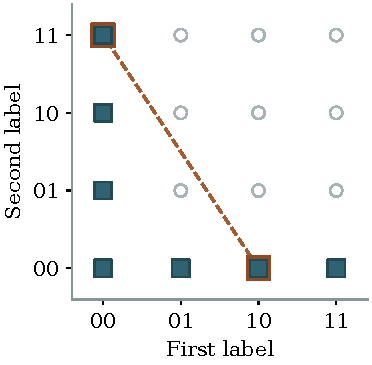
\includegraphics[width=.49\linewidth]{support-obstruction.pdf}
\caption{The coordinate support for \(k=2\). The linked basis labels are exchanged by the shift \((10,11)\). Every nonzero shift has such a pair on the two axes.}\label{fig:axes}
\end{figure}
Thus a uniform one-step guarantee first becomes possible at a dimension of order \(r^2\). This obstruction concerns the measurement rule itself.

\section{Odd prime local dimension}
Let \(D=p^n\) with \(p\) an odd prime. Encode entries in the power basis of \(\Q(\zeta_p)\), where \(\zeta_p=e^{2\pi i/p}\).
\begin{theorem}
For an explicit density matrix of rank \(r\) over \(\Q(\zeta_p)\), stabilizer membership and a convex decomposition for a member can be computed in \(2^{O(\log^2(r+1))}\operatorname{poly}(D,L)\) bit operations.
\end{theorem}
\begin{proof}
For a nonidentity Weyl label, choose a representative \(U\) of order \(p\) and let \(E_j\) be its spectral projections. Fourier orthogonality gives
\[
 \frac1p\sum_{j=0}^{p-1}\|p\Pi E_j\Pi-\Pi\|_F^2
 =\sum_{k=1}^{p-1}\|\Pi U^k\Pi\|_F^2 .
\]
For each \(k\ne0\bmod p\), the \(k\)-th power permutes the nonzero Weyl labels up to phase. Applying the Weyl twirl and removing the identity term, the mean of the right side over \(U\) is \((p-1)(Dr^2-r)/(D^2-1)\le(p-1)r^2/D\). If \(D>(p-1)r^2\), some \(p\Pi E_j\Pi\) differs from the identity on \(S\) by less than one in operator norm. This outcome is injective on \(S\) and has image in a space of dimension \(D/p\). Clifford decoding preserves stabilizer rays~\cite{hddm}. Each step sums along length-\(p\) orbits with root-of-unity factors, or selects coordinates for a diagonal measurement. In a length-\(p\) coefficient representation, multiplication by \(\zeta_p\) permutes coefficients. There are at most \(\log_pD\) rounds, so common-denominator coefficients, and their reductions to the power basis, have polynomial bit length.

The final space has \(m\le1+2\log_p r\) sites. Enumeration of Lagrangian bases and phase labels over \(\F_p\), followed by exact lifting and affine-support and quadratic-phase recognition, takes \(p^{O(m^2)}\operatorname{poly}(D,L)\) time. Since \(p\le D\), this has the stated bound. For \(D=1\) the assertion is immediate.

For the final feasibility test, use Gross's Wigner coordinates~\cite{gross}. After multiplying them by \(D\), each stabilizer column is the zero-one indicator of an affine Lagrangian. The problem is \(Ay=b,\ y\ge0\), with \(A\) integral and \(b\) in the real part of the cyclotomic field. Here is an explicit precision bound for reducing it to rational LP. Write \(d_0=D^2,\ H=d_0!\), choose \(Q\ge1\) clearing the denominators of \(b\), and choose an integer \(C_0\ge1\) bounding all conjugate moduli of the \(Qb_i\), for instance from the sum of the absolute coefficients. In an infeasible instance a vertex of the polytope \(A^Tz\ge0,\ -1\le z_i\le1\) satisfies \(z\cdot b<0\). By Cramer's rule this vertex has a common denominator \(d\le H\). The nonzero algebraic integer \(dQz\cdot b\) has conjugate moduli at most \(Hd_0 C_0\). Its field norm is a nonzero integer, so
\[
 -z\cdot b\ \ge\ \gamma
 :=\bigl[H Q(Hd_0 C_0)^{p-2}\bigr]^{-1}.
\]
Approximate \(b\) by a rational \(\widehat b\) to sup-norm accuracy \(\delta=\gamma/(4d_0)\) and test \(\|Ay-\widehat b\|_\infty\le\delta,\ y\ge0\). Exact feasibility implies feasibility of this system. A negative separating vertex rules out approximate feasibility, since \(2d_0\delta<\gamma\). The power-basis representation allows evaluation at \(e^{2\pi i/p}\) to the indicated polynomial bit precision. Deleting columns whenever feasibility persists leaves a minimal support. A dependence in that support would allow a positive coefficient to be reduced to zero, so the remaining columns are independent. Exact solution in the original field now recovers the probabilities.
\end{proof}

\section{Conclusion}
The support of a low-rank state can be compressed before its stabilizer vertices are listed. For qubits this yields both an exact decomposition on the face and a separator valid on the full polytope. The coordinate examples locate the worst-case scale of injective Pauli postselection within a constant factor. The same support compression extends to odd prime local dimension by averaging the Fourier components of the measurement outcomes.
\begingroup\small
\begin{thebibliography}{99}
\bibitem{ddm} J. Dehaene and B. De Moor, \href{https://arxiv.org/abs/quant-ph/0304125}{The Clifford group, stabilizer states, and linear and quadratic operations over \(\mathrm{GF}(2)\)}, \emph{Phys. Rev. A} 68 (2003), 042318.
\bibitem{bravyi} S. Bravyi, D. Browne, P. Calpin, E. Campbell, D. Gosset and M. Howard, \href{https://arxiv.org/abs/1808.00128}{Simulation of quantum circuits by low-rank stabilizer decompositions}, \emph{Quantum} 3 (2019), 181.
\bibitem{lb} L. Leone and L. Bittel, \href{https://arxiv.org/abs/2404.11652}{Stabilizer entropies are monotones for magic-state resource theory}, \emph{Phys. Rev. A} 110 (2024), L040403.
\bibitem{leo} L. Leone, J. Eisert and S. F. E. Oliviero, \href{https://arxiv.org/abs/2602.22330v2}{The unbearable hardness of deciding about magic}, arXiv:2602.22330v2 (2026).
\bibitem{tardos} \'E. Tardos, \href{https://doi.org/10.1287/opre.34.2.250}{A strongly polynomial algorithm to solve combinatorial linear programs}, \emph{Oper. Res.} 34 (1986), 250--256.
\bibitem{hddm} E. Hostens, J. Dehaene and B. De Moor, \href{https://arxiv.org/abs/quant-ph/0408190}{Stabilizer states and Clifford operations for systems of arbitrary dimensions, and modular arithmetic}, \emph{Phys. Rev. A} 71 (2005), 042315.
\bibitem{gross} D. Gross, \href{https://arxiv.org/abs/quant-ph/0602001}{Hudson's theorem for finite-dimensional quantum systems}, \emph{J. Math. Phys.} 47 (2006), 122107.
\end{thebibliography}
\endgroup
\end{document}
